\documentclass{article}
\usepackage{amsmath}
\usepackage{amssymb}
\usepackage{graphicx}
\author{Yichen ZHU}
\title{Compte rendu TP RLS}
\begin{document}
\maketitle

\paragraph{1.} On prend le mod\`ele source excitation pour cette \'etude de cas. Pendant la prononciation d'un son vois\'e, on a le son de la glotte qui repr\'esente le signal d'\'excitation $E(z)$ et le son provoqu\'e par les cordes vocales repr\'esente le signal de source $A(z)$ qui est en vrai un ``all pole filter". On a notre son vois\'e $X(z)$ repr\'esent\'e par le mod\`ele suivant :
\[
X(z) = \frac{E(z)}{A(z)}
\]
Ici on veut montrer que ce mod\`ele peut \^etre r\'ealis\'e par un algorithme de RLS. Le principe est de pr\'edire le scalaire $x_{n}$ \`a partir de son pass\'e c'est \`a dire les P derniers \'echantillons de $x$. Le r\'esidu ou l'erreur de pr\'ediction est bien \'equivalant au signal d'\'excitation. Ci dessous la justification : 
\\
\\On a le r\'esidu : $e_{n} = x_{n} - y^{T}_{n}\widehat{\theta}$ avec $\widehat{\theta}$ le filtre optimis\'e pour la pr\'ediction.
\\On remplace $y^{T}_{n}$ par les pass\'es de $x_{n}$ : 
\begin{eqnarray*}
e_{n} &=& x_{n} - x^{T}_{n-1}\widehat{\theta} \\
      &=& x_{n} + \sum^{P}_{i=1}x_{n-i}\widehat{\theta}_{i} \\
			&=& \sum^{P}_{i=0}x_{n-i}\widehat{\theta}_{i} \\
\end{eqnarray*}	
\\On peut faire entrer $x_{n}$ dans la somme car le terme $\theta_{0}=1$
\\Ensuite, on prend sa transform\'ee en $Z$ : 
\begin{eqnarray*}
E(z) &=& \sum_{n=0}^{P}x_{n}z^{n}\sum_{n=0}^{P}\theta_{n}z^{n} \\
     &=&  X(z)A(z) \\
\end{eqnarray*}
Avec $A(z)$ un polyn\^ome dont les coefficients sont $(-\theta_{0},-\theta_{1},\cdots,-\theta_{p})$

\paragraph{2.} On fait tourner l'algorithme de RLS. On fait afficher le signal du r\'esidu : \\
\begin{figure}[h]
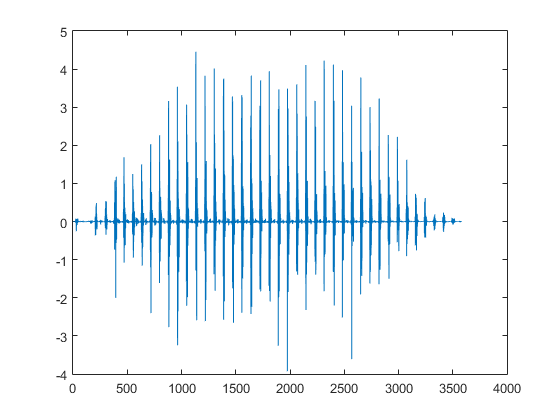
\includegraphics[scale=0.25]{residu_a.png} 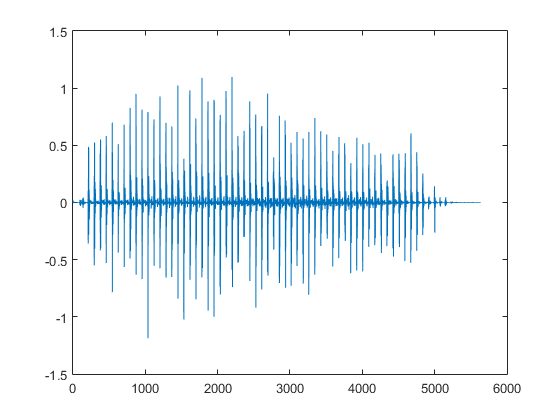
\includegraphics[scale=0.25]{residu_o.png} 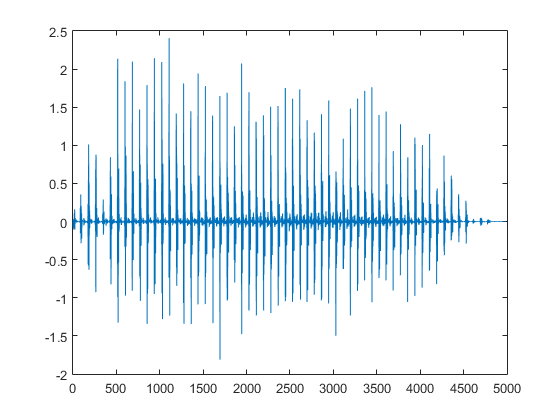
\includegraphics[scale=0.25]{residu_e.png} 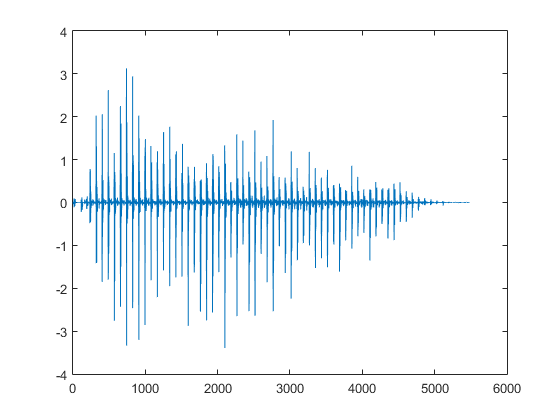
\includegraphics[scale=0.25]{residu_i.png} 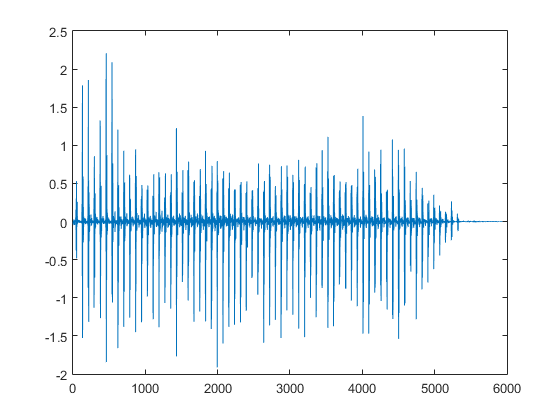
\includegraphics[scale=0.25]{residu_u.png}
\caption{r\'esidus des signaux vois\'es a,o,e,i,u}
\end{figure} 
\\On voit bien que les r\'esidus de diff\'errents signaux vois\'es ont la m\^eme fr\'equence, ensuite si on compare le r\'esidu avec le signal vois\'e, on prend l'exemple de ``a" :
\begin{figure}[h] 
\begin{center}
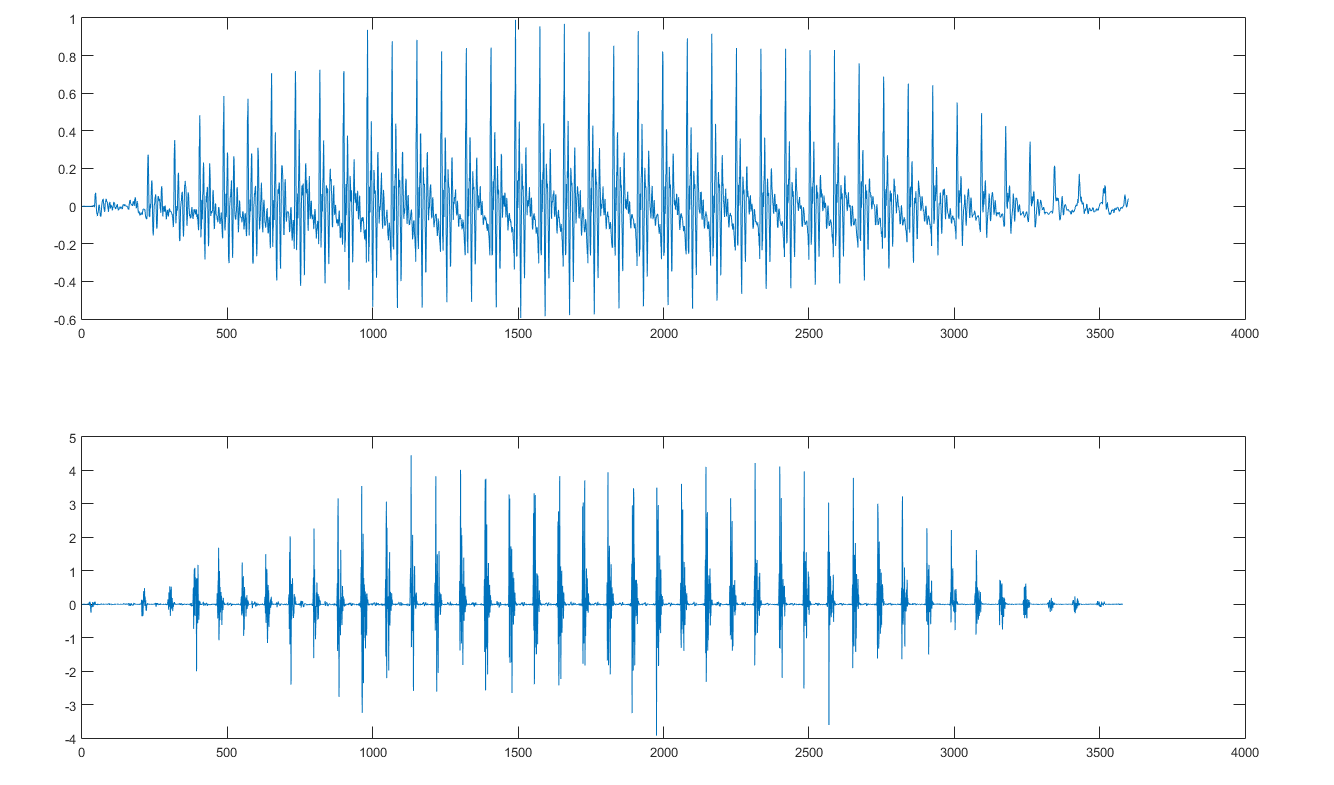
\includegraphics[scale=0.3]{residual.png}
\caption{le signal vois\'e et le r\'esidu}
\end{center}
\end{figure}
\\On remarque que le signal vois\'e est bien le signal de r\'esidu modul\'e avec un autre signal source.
\\Apr\`es, on s'int\'eresse \`a \'ecouter le signal r\'esidu. On entend un bruit d'impultion de certaine fr\'equence. Ce signal est \`a peu pr\`es pareil pour tous les signaux vois\'es.
\paragraph{3.} On s'int\'eresse maintenant \`a la recherche de la fr\'equence de pitch. On propose ici trois m\'ethodes pour en faire.
\subparagraph{i.} On utilise la fonction ``spectro" pour relever le spectrogramme du signal.
\begin{figure}[!h] 
\begin{center}
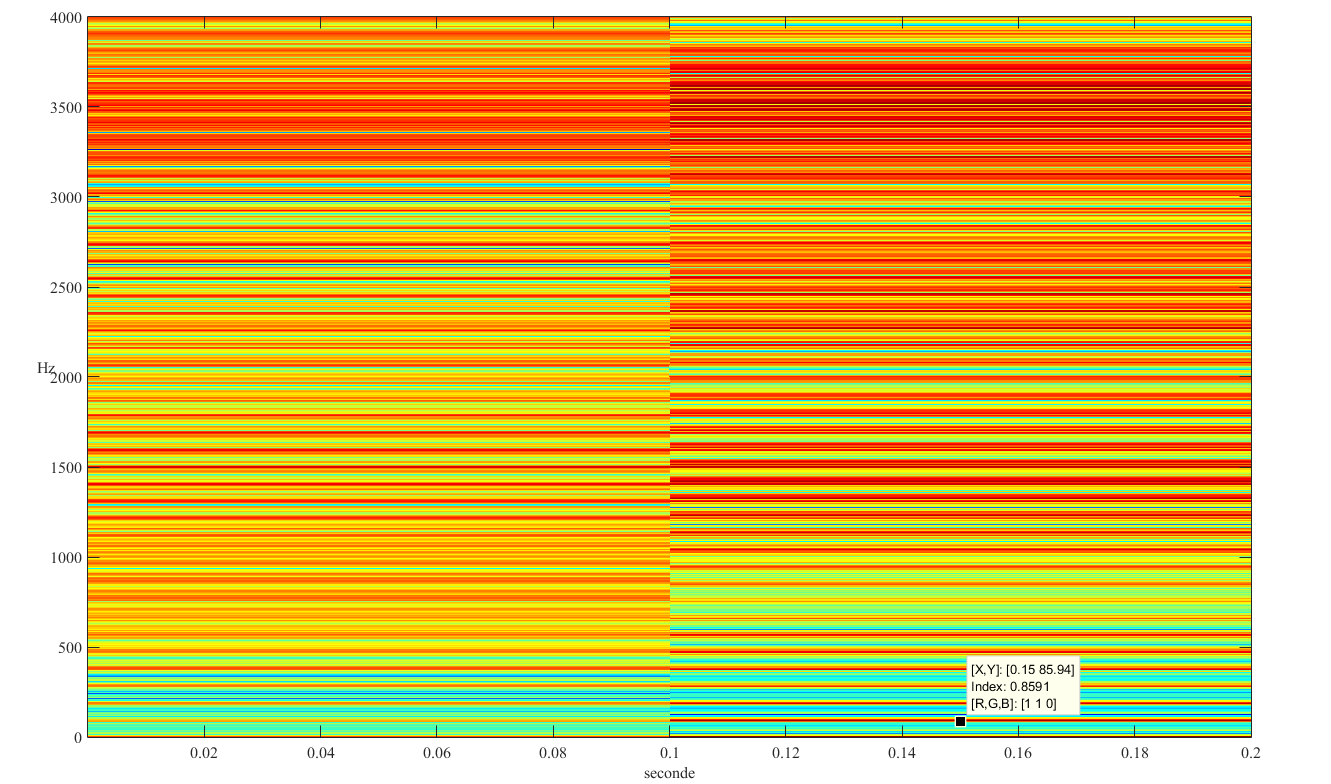
\includegraphics[scale=0.25]{spectro_a.png}
\caption{spectrogramme du r\'esidu}
\end{center}
\end{figure}
\\On voit bien le premier pic (celui qui est plus fonc\'e) appara\^it \`a 85.94Hz. On a donc la fr\'equence du pitch \`a cette fr\'equence.
\subparagraph{ii.} On fait afficher le p\'eriodogramme du r\'esidu.
\begin{figure}[!h] 
\begin{center}
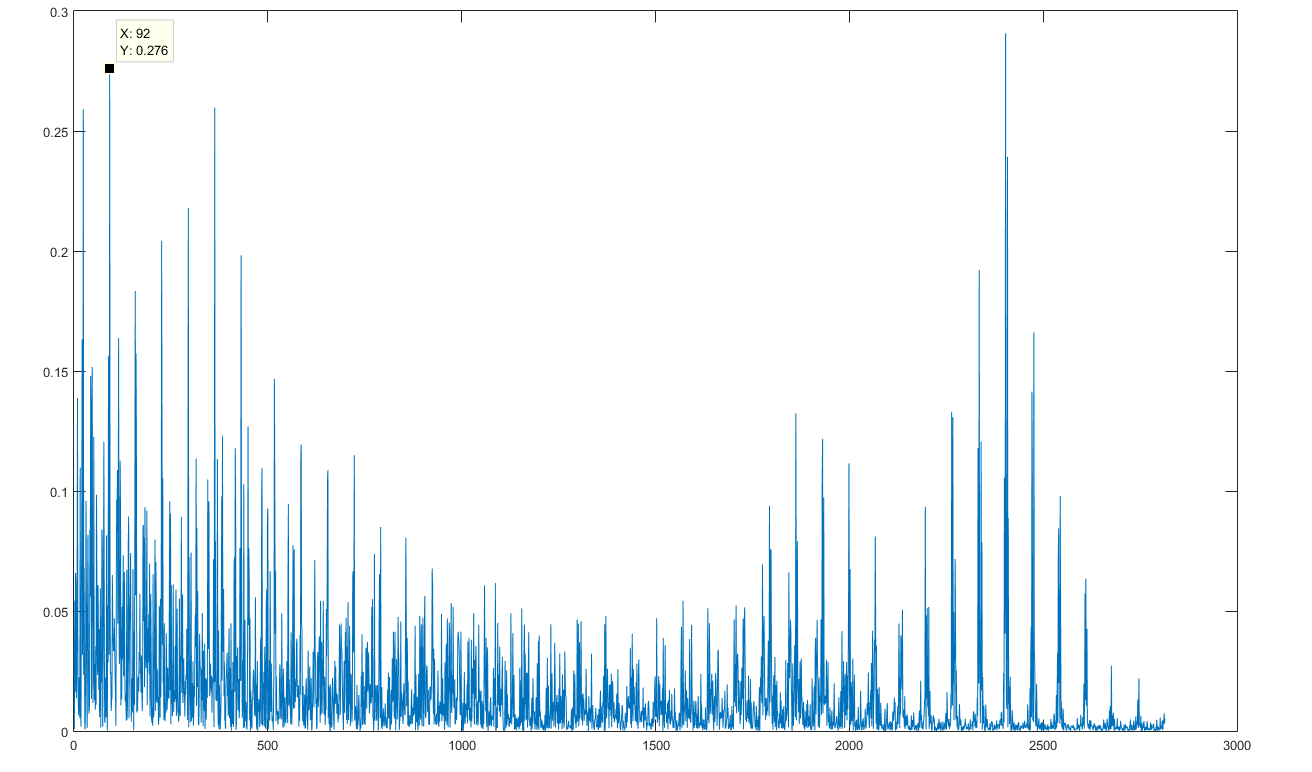
\includegraphics[scale=0.25]{periodo.png}
\caption{p\'eriodogramme du r\'esidu}
\end{center}
\end{figure}
\\On trouve la fondamentale \`a 92Hz.
\subparagraph{iii.} On utilise la fonction ``autocorr" pour compter la longueur de l'\'ecart entre les pics. 
\begin{figure}[!h] 
\begin{center}
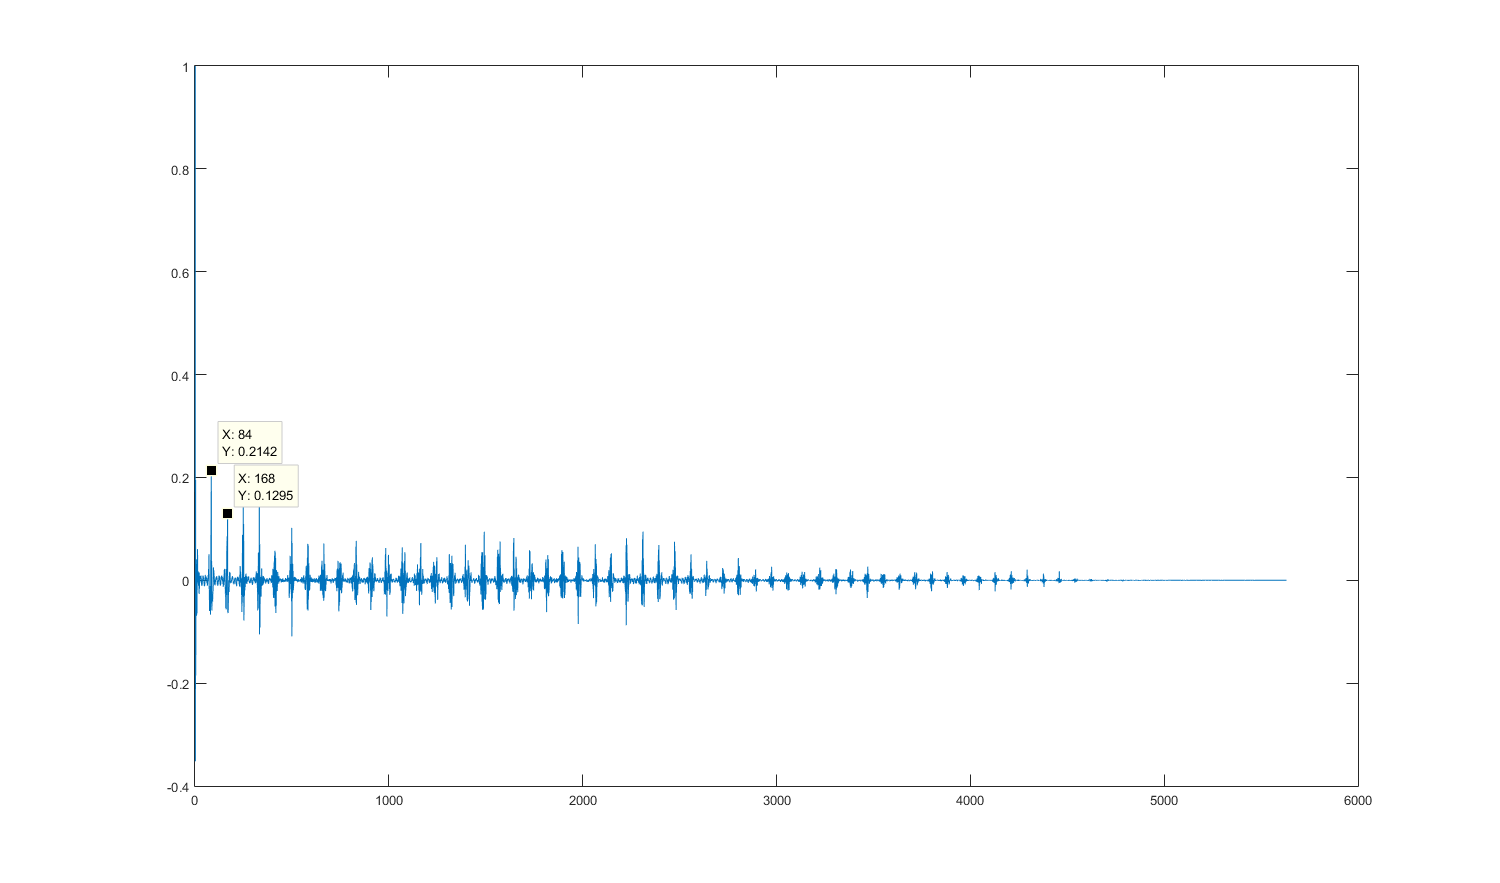
\includegraphics[scale=0.25]{autocorr.png}
\caption{autocorr\'elation du r\'esidu}
\end{center}
\end{figure}
\\On a donc la fr\'equence du pitch $168-84=84Hz$

\end{document}